\uuid{4Fy0}
\exo7id{5524}
\titre{exo7 5524}
\auteur{rouget}
\organisation{exo7}
\datecreate{2010-07-15}
\isIndication{false}
\isCorrection{true}
\chapitre{Courbes planes}
\sousChapitre{Courbes paramétrées}
\module{Géométrie}
\niveau{L2}
\difficulte{}

\contenu{
\texte{
Construire les courbes de paramétrisations :
}
\begin{enumerate}
    \item \question{$\left\{\begin{array}{l}
x=\frac{t^3}{(t+1)^2(t-1)}\\
y=\frac{t^2}{t^2-1}
\end{array}\right.$}
\reponse{\textbf{Domaine d'étude.}
$M(t)$ existe si et seulement si $t\notin\{-1,1\}$. Sinon, il n'y a pas de symétrie particulière (la fonction $y$ est effectivement paire, mais $x$ n'est ni paire ni impaire).

\textbf{Dérivée.} Pour $t\in]-1,1[\setminus\{0\}$,

\begin{align*}\ensuremath
x'(t)&=x(t)(3\ln|t|-2\ln|t+1|-\ln|t-1|)'=\frac{t^3}{(t+1)^2(t-1)}(\frac{3}{t}-\frac{2}{t+1}-\frac{1}{t-1})\\
 &=\frac{t^3}{(t+1)^2(t-1)}\frac{3(t^2-1)-2(t^2-t)-(t^2+t)}{t(t+1)(t-1)}=\frac{t^2(t-3)}{(t+1)^3(t-1)^2},
\end{align*}

et

$$y'(t)=\frac{2t(t^2-1)-2t(t^2)}{(t^2-1)^2}=\frac{-2t}{(t^2-1)^2},$$

ce qui reste vrai par continuité de $x$ et $y$ en $0$.

\textbf{Etude des points singuliers.} Pour $t\in]-1,1[$, $\overrightarrow{\frac{dM}{dt}}(t)=\vec{0}\Leftrightarrow t=0$. $M(0)=(0,0)$ est l'unique point singulier. Pour $t\in]-1,1[\setminus\{0\}$,

$$\frac{y(t)-y(0)}{x(t)-x(0)}=\frac{t^2}{t^2-1}\frac{(t+1)^2(t-1)}{t^3}=\frac{t+1}{t}.$$

Par suite, $\frac{y(t)-y(0)}{x(t)-x(0)}$ tend vers $+\infty$ quand $t$ tend vers $0$ par valeurs supérieures et vers $-\infty$ quand $t$ tend vers $0$ par valeurs inférieures. La tangente en $M(0)$ est dirigée par $\vec{j}$ et d'autre part, $M(0)$ est un point de rebroussement de première espèce.

\textbf{Etude quand $t$ tend vers $\pm\infty$.} Quand $t$ tend vers $\pm\infty$, $M(t)$ tend vers le point $(1,1)$. On prolonge la courbe en posant $M(\infty)=1,1)$. On a alors

$$\frac{y(t)-y(\infty)}{x(t)-x(\infty)}=(\frac{t^2}{t^2-1}-1)(\frac{t^3}{(t+1)^2(t-1)}-1)^{-1}=\frac{1}{t^2-1}
\frac{(t+1)^2(t-1)}{-t^2+t+1}=\frac{t+1}{-t^2+t+1}\sim-\frac{1}{t}.$$

Cette expression tend donc vers $0$ quand $t$ tend vers $\pm\infty$ et la tangente en $M(\infty)$ est dirigée par $\vec{i}$.

\textbf{Etude quand $t$ tend vers 1.} Quand $t$ tend vers $1$, $x(t)\sim{1}{4(t-1)}$ et $y(t)\sim\frac{1}{2(t-1)}$. Donc, $x$ et $y$ tendent vers l'inifini et il y a branche infinie. De plus, $\frac{y(t)}{x(t)}\sim2$. Puis,

$$y(t)-2x(t)=\frac{t^2}{t^2-1}-2\frac{t^3}{(t+1)^2(t-1)}=\frac{t^2(t+1)-2t^3}{(t+1)^2(t-1)}=-\frac{t^2}{(t+1)^2}.$$

Cette dernière expression tend vers $-\frac{1}{4}$ et la droite $(\Delta)$ d'équation $y=2x-\frac{1}{4}$ est asymptote à la courbe.

\textbf{Etude quand $t$ tend vers -1.} Quand $t$ tend vers $1$, $x(t)\sim{1}{2(t+1)^2}$ et $y(t)\sim\frac{-1}{2(t+1)}$. Donc, $x$ et $y$ tendent vers l'inifini et il y a branche infinie. De plus, $\frac{y(t)}{x(t)}\sim-(t+1)$. Par suite, $\frac{y(t)}{x(t)}$ tend vers $0$ quand $t$ tend vers $-1$. La courbe admet une barnche parabolique de direction $(Ox)$.

\textbf{Variations conjointes de $x$ et $y$.} On rappelle que pour $t\in\Rr\setminus\{-1,1\}$, $x'(t)=\frac{t^2(t-3)}{(t+1)^3(t-1)^2}$ et $y'(t)=\frac{-2t}{(t^2-1)^2}$. On en déduit le tableau suivant~:

$$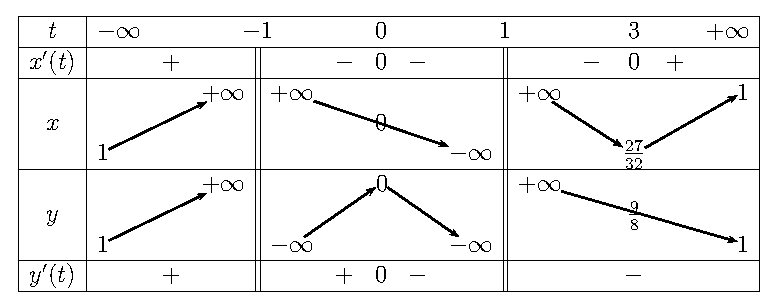
\includegraphics{../images/4Fy0-1}$$


On peut noter que la tangente en $M(3)$ est dirigée par le vecteur $\vec{j}$. Voir graphique page suivante.

$$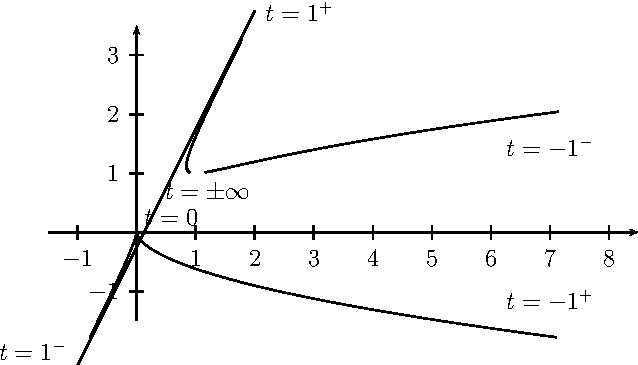
\includegraphics{../images/4Fy0-2}$$



Dans la suite de cet exercice, je ne détaillerai que très peu ou pas du tout l'étude de la courbe.}
    \item \question{$\left\{\begin{array}{l}
x=(t+2)e^{1/t}\\
y=(t-2)e^{1/t}
\end{array}\right.$}
\reponse{$$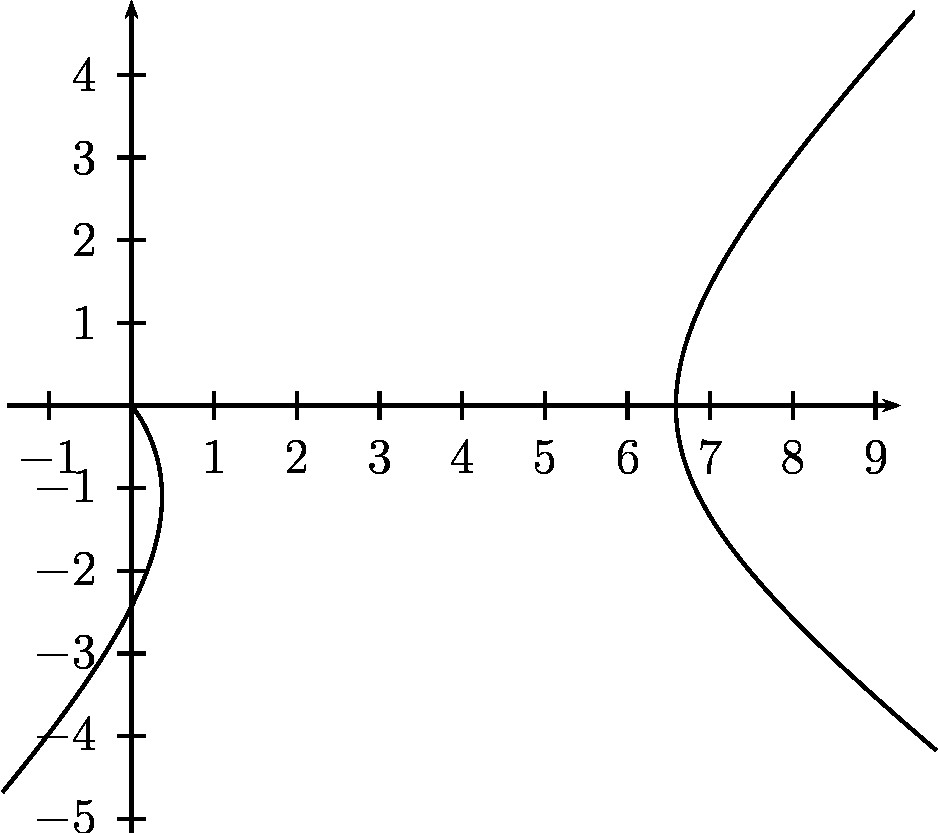
\includegraphics{../images/4Fy0-3}$$}
    \item \question{$\left\{\begin{array}{l}
x=(t-1)\ln(|t|)\\
y=(t+1)\ln(|t|)
\end{array}\right.$}
\reponse{$$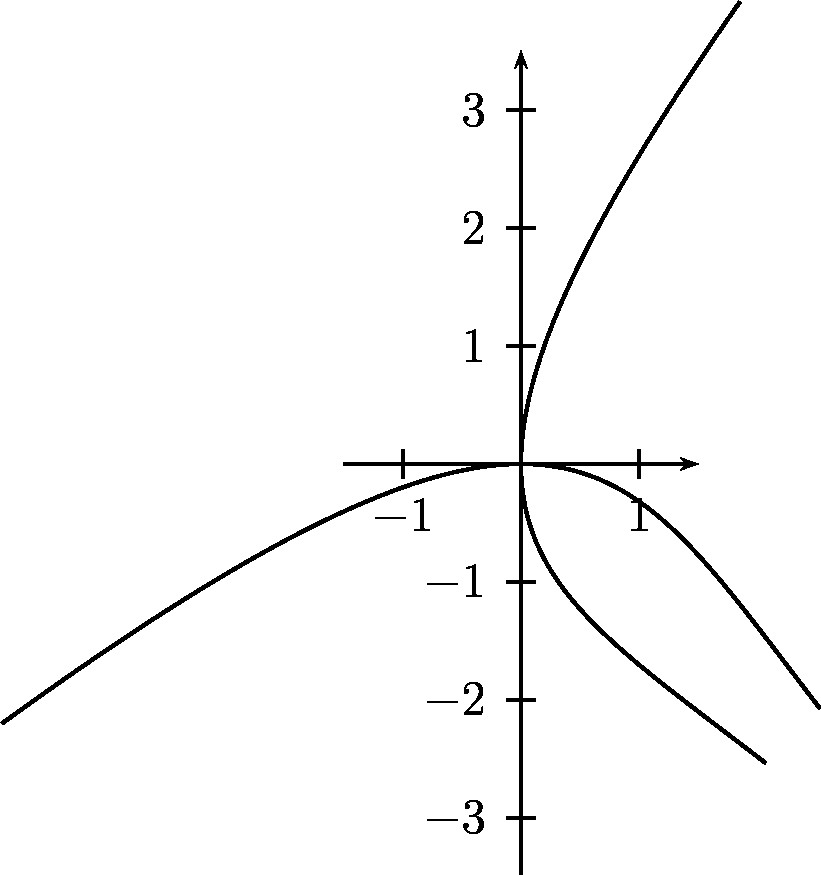
\includegraphics{../images/4Fy0-4}$$}
    \item \question{$\left\{\begin{array}{l}
x=\frac{2t}{1+t^2}\\
y=\frac{t+2}{1-t^2}
\end{array}\right.$}
\reponse{$\left\{\begin{array}{l}
x=\frac{2t}{1+t^2}\\
y=\frac{t+2}{1-t^2}
\end{array}\right.$

$$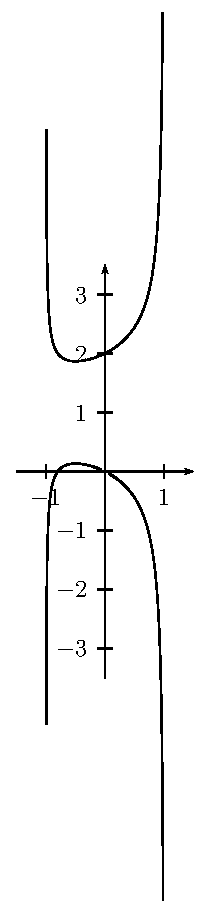
\includegraphics{../images/4Fy0-5}$$}
    \item \question{$\left\{\begin{array}{l}
x=\frac{t}{t^2-1}\\
y=\frac{t+2}{(t-1)^2}
\end{array}\right.$}
\reponse{$$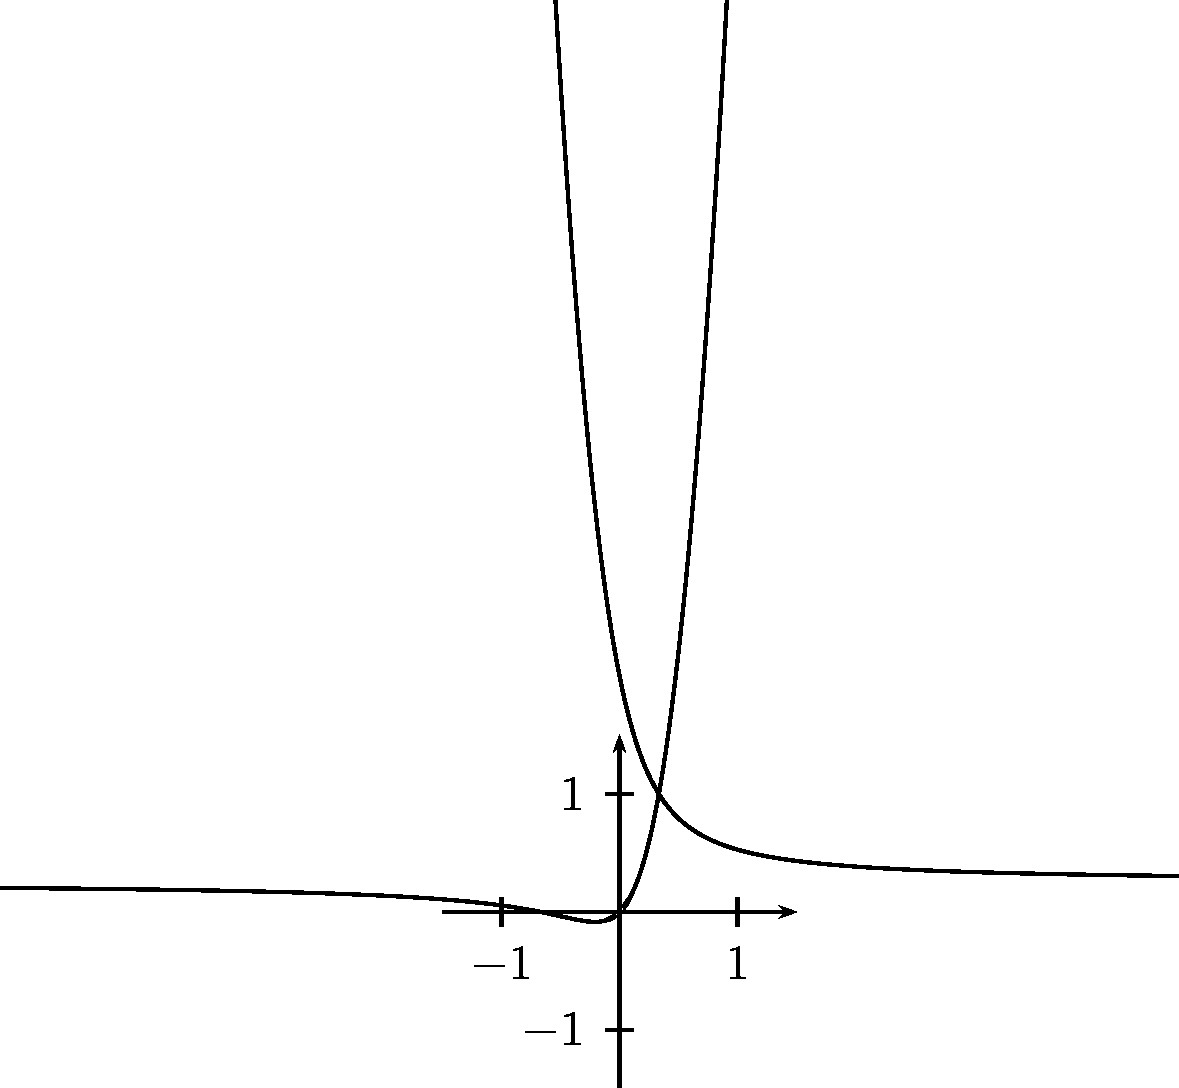
\includegraphics{../images/4Fy0-6}$$}
    \item \question{$\left\{\begin{array}{l}
x=\frac{t^3}{t^2-9}\\
y=\frac{t(t-2)}{t-3}
\end{array}\right.$}
\reponse{$\left\{\begin{array}{l}
x=\frac{t^3}{t^2-9}\\
y=\frac{t(t-2)}{t-3}
\end{array}\right.$

$$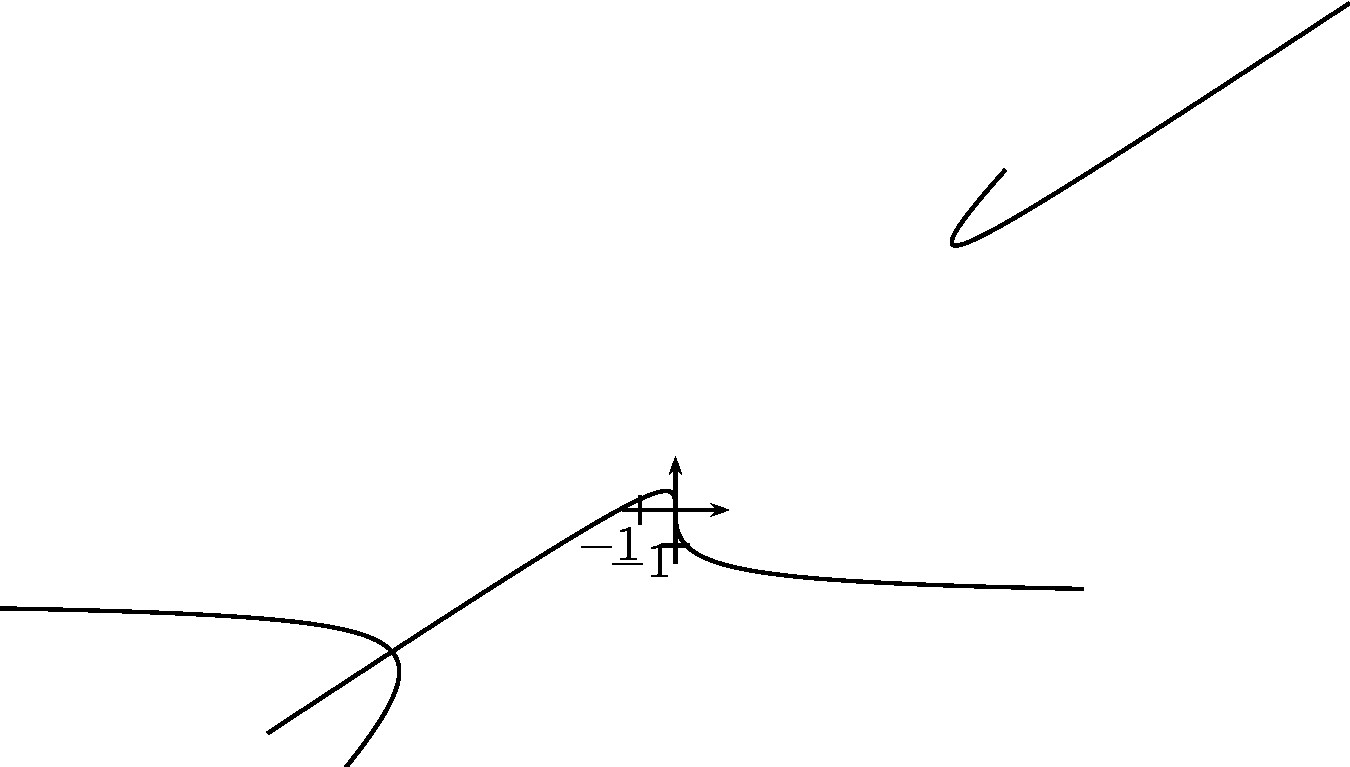
\includegraphics{../images/4Fy0-7}$$}
    \item \question{$\left\{\begin{array}{l}
x=\frac{t^3}{1+3t}\\
y=\frac{3t^2}{1+3t}
\end{array}\right.$}
\reponse{$\left\{\begin{array}{l}
x=\frac{t^3}{1+3t}\\
y=\frac{3t^2}{1+3t}
\end{array}\right.$

$$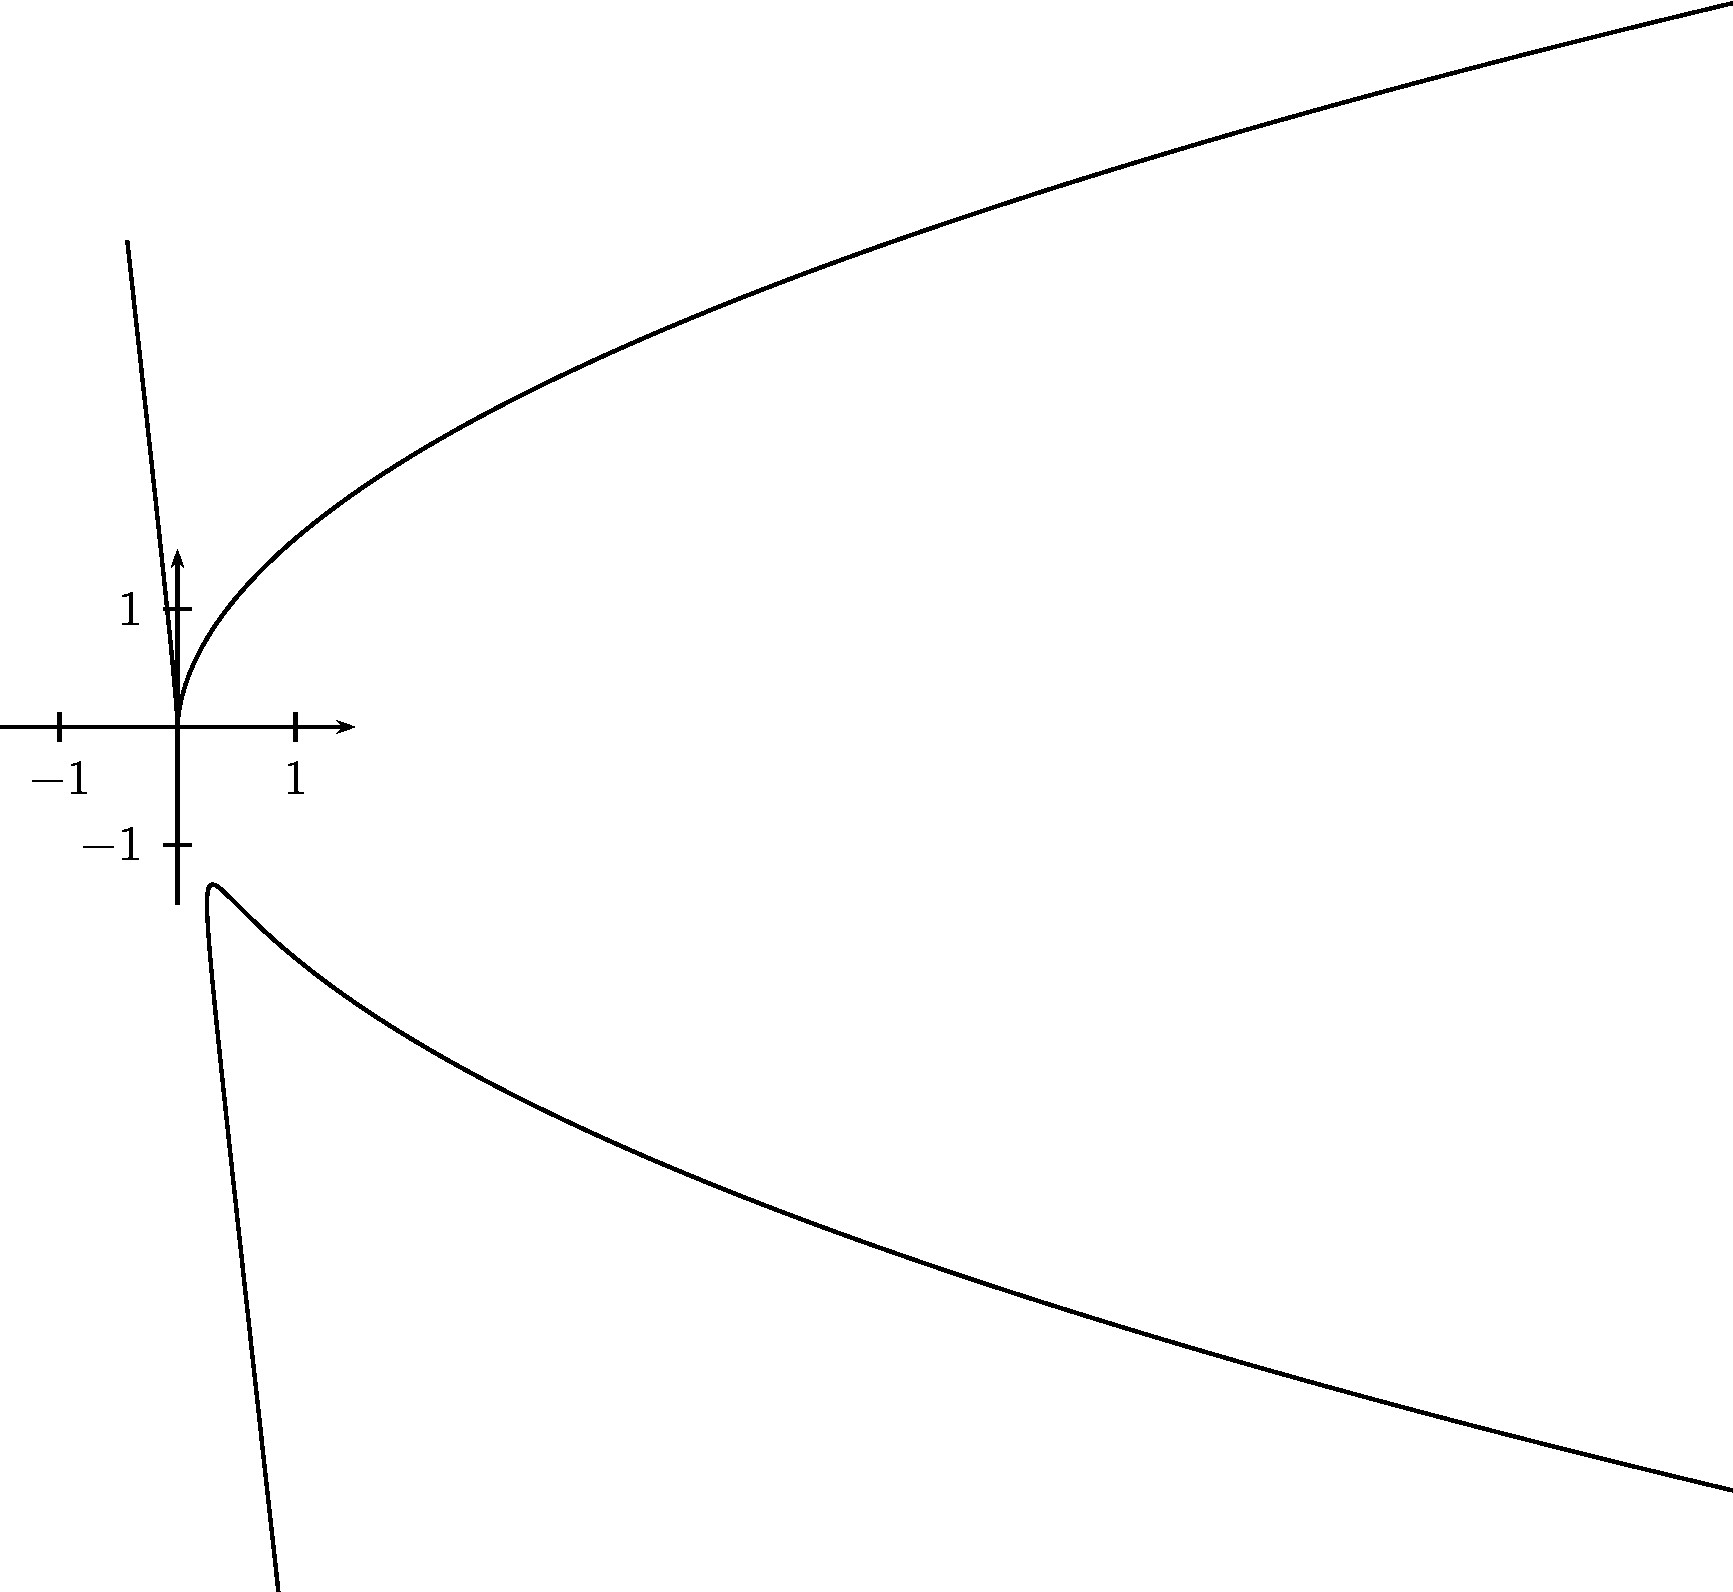
\includegraphics{../images/4Fy0-8}$$}
    \item \question{$\left\{\begin{array}{l}
x=t^2+t^3\\
y=t^2+t^3-2t^4-2t^5
\end{array}\right.$}
\reponse{$\left\{\begin{array}{l}
x=t^2+t^3\\
y=t^2+t^3-2t^4-2t^5
\end{array}\right.$

$$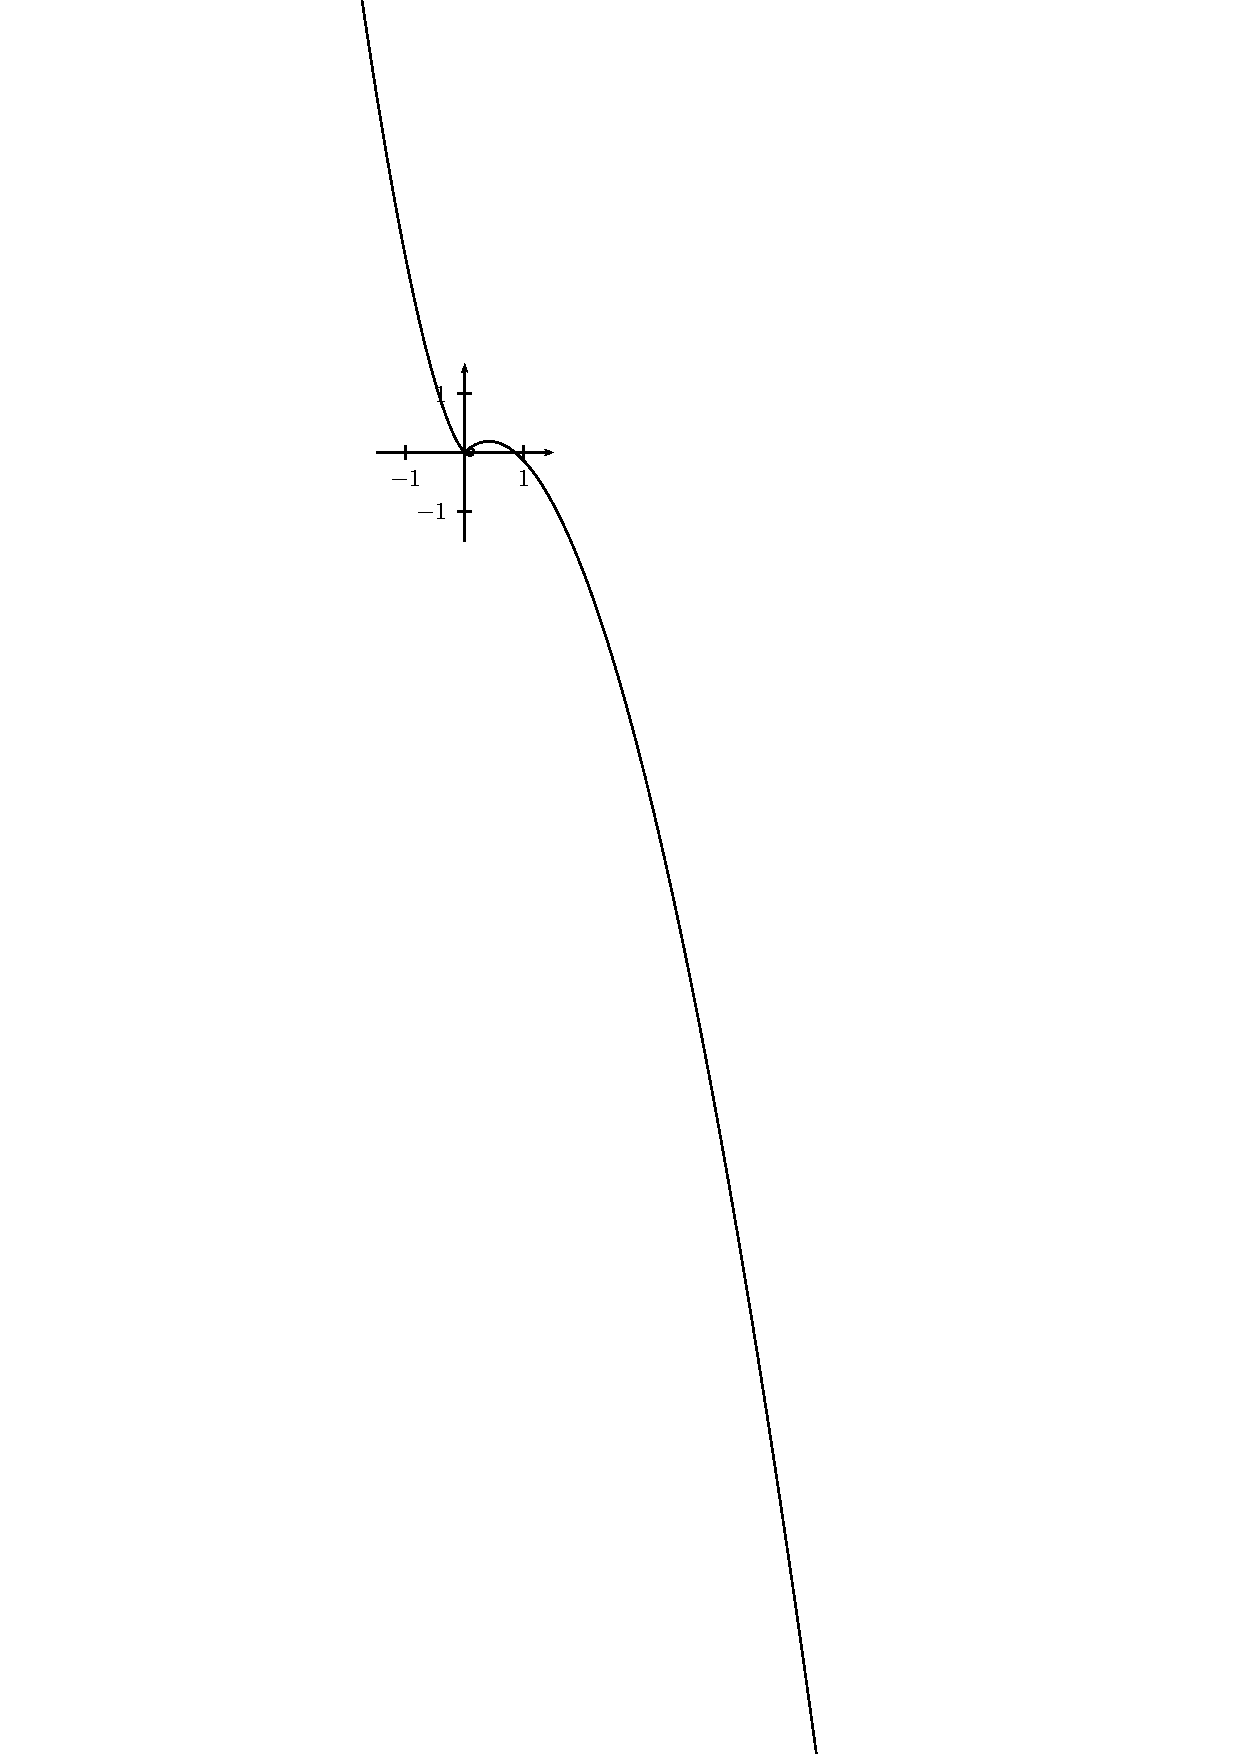
\includegraphics{../images/4Fy0-9}$$}
\end{enumerate}
}
